% !TEX program = lualatex
% !TEX TS-program = lualatex
\documentclass[10pt,aspectratio=169]{beamer}
% --- Engine: LuaLaTeX (or XeLaTeX) ---
% Build:  cd Slides && latexmk main.tex      (driven by .latexmkrc -> lualatex)
% Or:     lualatex main.tex && lualatex main.tex
\usepackage{fontspec}
% Use the TeX Live-bundled OTF files (filename prefix, no space).
\setsansfont{FiraSans}[
  Extension      = .otf,
  UprightFont    = *-Book,
  ItalicFont     = *-BookItalic,
  BoldFont       = *-SemiBold,
  BoldItalicFont = *-SemiBoldItalic,
]
\setmonofont{FiraMono}[
  Extension   = .otf,
  UprightFont = *-Regular,
  BoldFont    = *-Bold,
]
\usepackage{graphicx}
\usepackage{booktabs}
\usepackage{tikz}
\usetikzlibrary{positioning,arrows.meta}
\usepackage{xcolor}
\usepackage{tabularx}

% Theme: Metropolis (flat, modern) + HCMUT-blue accent
\usetheme[progressbar=frametitle, block=fill, sectionpage=none]{metropolis}
\definecolor{hcmutblue}{HTML}{0072BA}
\definecolor{hcmutblueDark}{HTML}{004C7A}
\setbeamercolor{normal text}{fg=black!85,bg=white}
\setbeamercolor{alerted text}{fg=hcmutblue}
\setbeamercolor{progress bar}{fg=hcmutblue, bg=hcmutblue!20}
\setbeamercolor{title separator}{fg=hcmutblue}
\setbeamercolor{progress bar in head/foot}{fg=hcmutblue}
\setbeamercolor{progress bar in section page}{fg=hcmutblue}
\setbeamercolor{frametitle}{bg=hcmutblueDark, fg=white}
\setbeamercolor{section in toc}{fg=hcmutblueDark}
\setbeamerfont{frametitle}{size=\large, series=\bfseries}

% Reuse images from parent report
\graphicspath{{../Images/}{../Images/experiments/}{../Images/techstack/}}

\title[LSH Book Recommendation]{Hệ thống gợi ý sách tương tự dựa trên LSH}
\subtitle{Locality-Sensitive Hashing + Similarity Join trên Apache Spark}
\author[Nhóm LSH]{[Tên thành viên 1] \and [Tên thành viên 2] \and [Tên thành viên 3]}
\institute[HCMUT]{Khoa Khoa học và Kỹ thuật Máy tính \\ Trường Đại học Bách khoa, ĐHQG-HCM}
\date{Mini Project Dữ liệu lớn --- HK2 2025-2026}

\begin{document}

% ============================================================
% Slide 1 --- Title (custom layout, logo top-right)
% ============================================================
\begin{frame}[plain]
  % HCMUT logo overlay in top-right corner
  \begin{tikzpicture}[remember picture, overlay]
    \node[anchor=north east, inner sep=15pt]
      at (current page.north east)
      {
\includegraphics[width=1.6cm]{bachkhoa_logo.png}};
  \end{tikzpicture}

  \vspace*{1.6cm}
  {\small\color{hcmutblueDark}\textbf{Mini Project Dữ liệu lớn --- HK2 2025-2026}\par}
  \vspace{0.2cm}
  {\footnotesize Khoa Khoa học và Kỹ thuật Máy tính \\
   Trường Đại học Bách khoa, ĐHQG-HCM\par}

  \vspace{1.6cm}
  {\LARGE\bfseries\color{hcmutblueDark} Hệ thống gợi ý sách tương tự dựa trên LSH\par}
  \vspace{0.35cm}
  {\large Locality-Sensitive Hashing + Similarity Join trên Apache Spark\par}

  \vspace{0.5cm}
  {\color{hcmutblue}\rule{0.85\textwidth}{0.6pt}\par}

  \vspace{0.6cm}
  {\footnotesize\textbf{Nhóm thực hiện:}\par}
  \vspace{0.1cm}
  {\normalsize [Tên thành viên 1] \quad\textbullet\quad [Tên thành viên 2] \quad\textbullet\quad [Tên thành viên 3]\par}
\end{frame}

% ============================================================
% Slide 2 --- Outline
% ============================================================
\begin{frame}{Mục lục}
  \tableofcontents
\end{frame}

% ============================================================
% PART 1 --- [Thành viên 1]: Bài toán & Tech Stack
% ============================================================
\begin{frame}[plain]
  \vfill
  \centering
  {\Huge\color{hcmutblue}\textbf{Phần 1}}\par
  \vspace{0.5em}
  {\Large Bài toán \& Tech Stack}\par
  \vspace{1em}
  {\large Trình bày: \textbf{[Tên thành viên 1]}}\par
  \vfill
\end{frame}

\section{Bài toán Similarity Search}

\begin{frame}{Bài toán Similarity Search}
  Cho bộ tài liệu $D = \{d_1, d_2, \ldots, d_N\}$, tìm cặp $(d_i, d_j)$ có
  $$J(d_i, d_j) = \frac{|d_i \cap d_j|}{|d_i \cup d_j|} \geq t$$

  \textbf{Thách thức:}
  \begin{itemize}
    \item Brute-force pairwise: $O(N^2)$ --- bất khả thi với hàng triệu tài liệu.
    \item Cần phương pháp \emph{xấp xỉ} có chi phí gần tuyến tính.
  \end{itemize}

  \vfill
  \textbf{Giải pháp:} \textbf{Locality-Sensitive Hashing (LSH)} --- hash các tài liệu sao cho \emph{tài liệu giống nhau có xác suất cao rơi vào cùng bucket}.
\end{frame}

\section{Mục tiêu đề tài}

\begin{frame}{Mục tiêu đề tài}
  Xây dựng hệ thống \textbf{Similar Book Recommendation} dựa trên LSH + MRS Join (Map-Reduce based Similarity Join).

  \begin{enumerate}
    \item \textbf{Pipeline end-to-end:} raw text $\rightarrow$ tiền xử lý $\rightarrow$ MinHash $\rightarrow$ LSH index $\rightarrow$ truy vấn Top-K.
    \item \textbf{Triển khai phân tán:} Apache Spark trên cluster Hadoop / Databricks.
    \item \textbf{Đánh giá toàn diện:} Recall, Precision, F1, Speedup, Scalability, Selectivity.
    \item \textbf{Phân tích thực tế:} đặc tính LSH ở các quy mô dữ liệu khác nhau.
  \end{enumerate}

  \vfill
  \textbf{Phạm vi:} Project Gutenberg (English plain text), Jaccard similarity, content-based.
\end{frame}

\section{Kiến trúc tổng quan}

\begin{frame}{Pipeline 5 giai đoạn}
  \begin{center}
  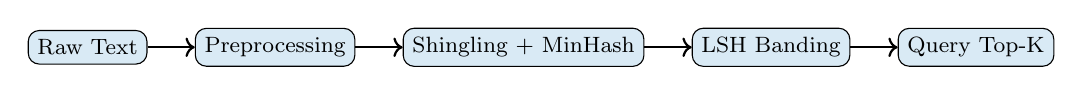
\begin{tikzpicture}[node distance=1cm and 0.6cm, every node/.style={font=\footnotesize, draw, rounded corners, fill=hcmutblue!15}]
    \node (raw)   {Raw Text};
    \node (clean) [right=of raw] {Preprocessing};
    \node (sig)   [right=of clean] {Shingling + MinHash};
    \node (lsh)   [right=of sig] {LSH Banding};
    \node (q)     [right=of lsh] {Query Top-K};
    \draw[->, thick] (raw)   -- (clean);
    \draw[->, thick] (clean) -- (sig);
    \draw[->, thick] (sig)   -- (lsh);
    \draw[->, thick] (lsh)   -- (q);
  \end{tikzpicture}
  \end{center}

  \vfill
  \begin{itemize}
    \item \textbf{Storage:} HDFS (thiết kế) / Databricks Volumes (thực thi).
    \item \textbf{Format trung gian:} Apache Parquet (columnar).
    \item \textbf{Engine:} Apache Spark (PySpark).
  \end{itemize}
\end{frame}

\section{Tech Stack \& Pivot HDFS $\rightarrow$ Databricks}

\begin{frame}{Tech Stack \& câu chuyện pivot}
  \begin{columns}[T]
    \column{0.48\textwidth}
    \textbf{Kế hoạch ban đầu:}
    \begin{itemize}
      \item Cluster Hadoop 3 nút
      \item HDFS + Spark on YARN
      \item Dataset 3K--10K sách
    \end{itemize}
    \vspace{0.4em}
    \textbf{Vấn đề:} Cloud credits không được duyệt đúng tiến độ.

    \column{0.48\textwidth}
    \textbf{Pivot:} \textbf{Databricks Free Edition (Serverless)}
    \begin{itemize}
      \item Auto-mount Git repo qua \texttt{/Workspace/Repos/}
      \item Không cần dựng cluster
      \item Notebook UX
    \end{itemize}
    \vspace{0.4em}
    \textbf{Đánh đổi:} mất \texttt{spark.sparkContext}, driver memory hẹp $\rightarrow$ TN3 phải scale-down.
  \end{columns}

  \vfill
  \begin{center}
    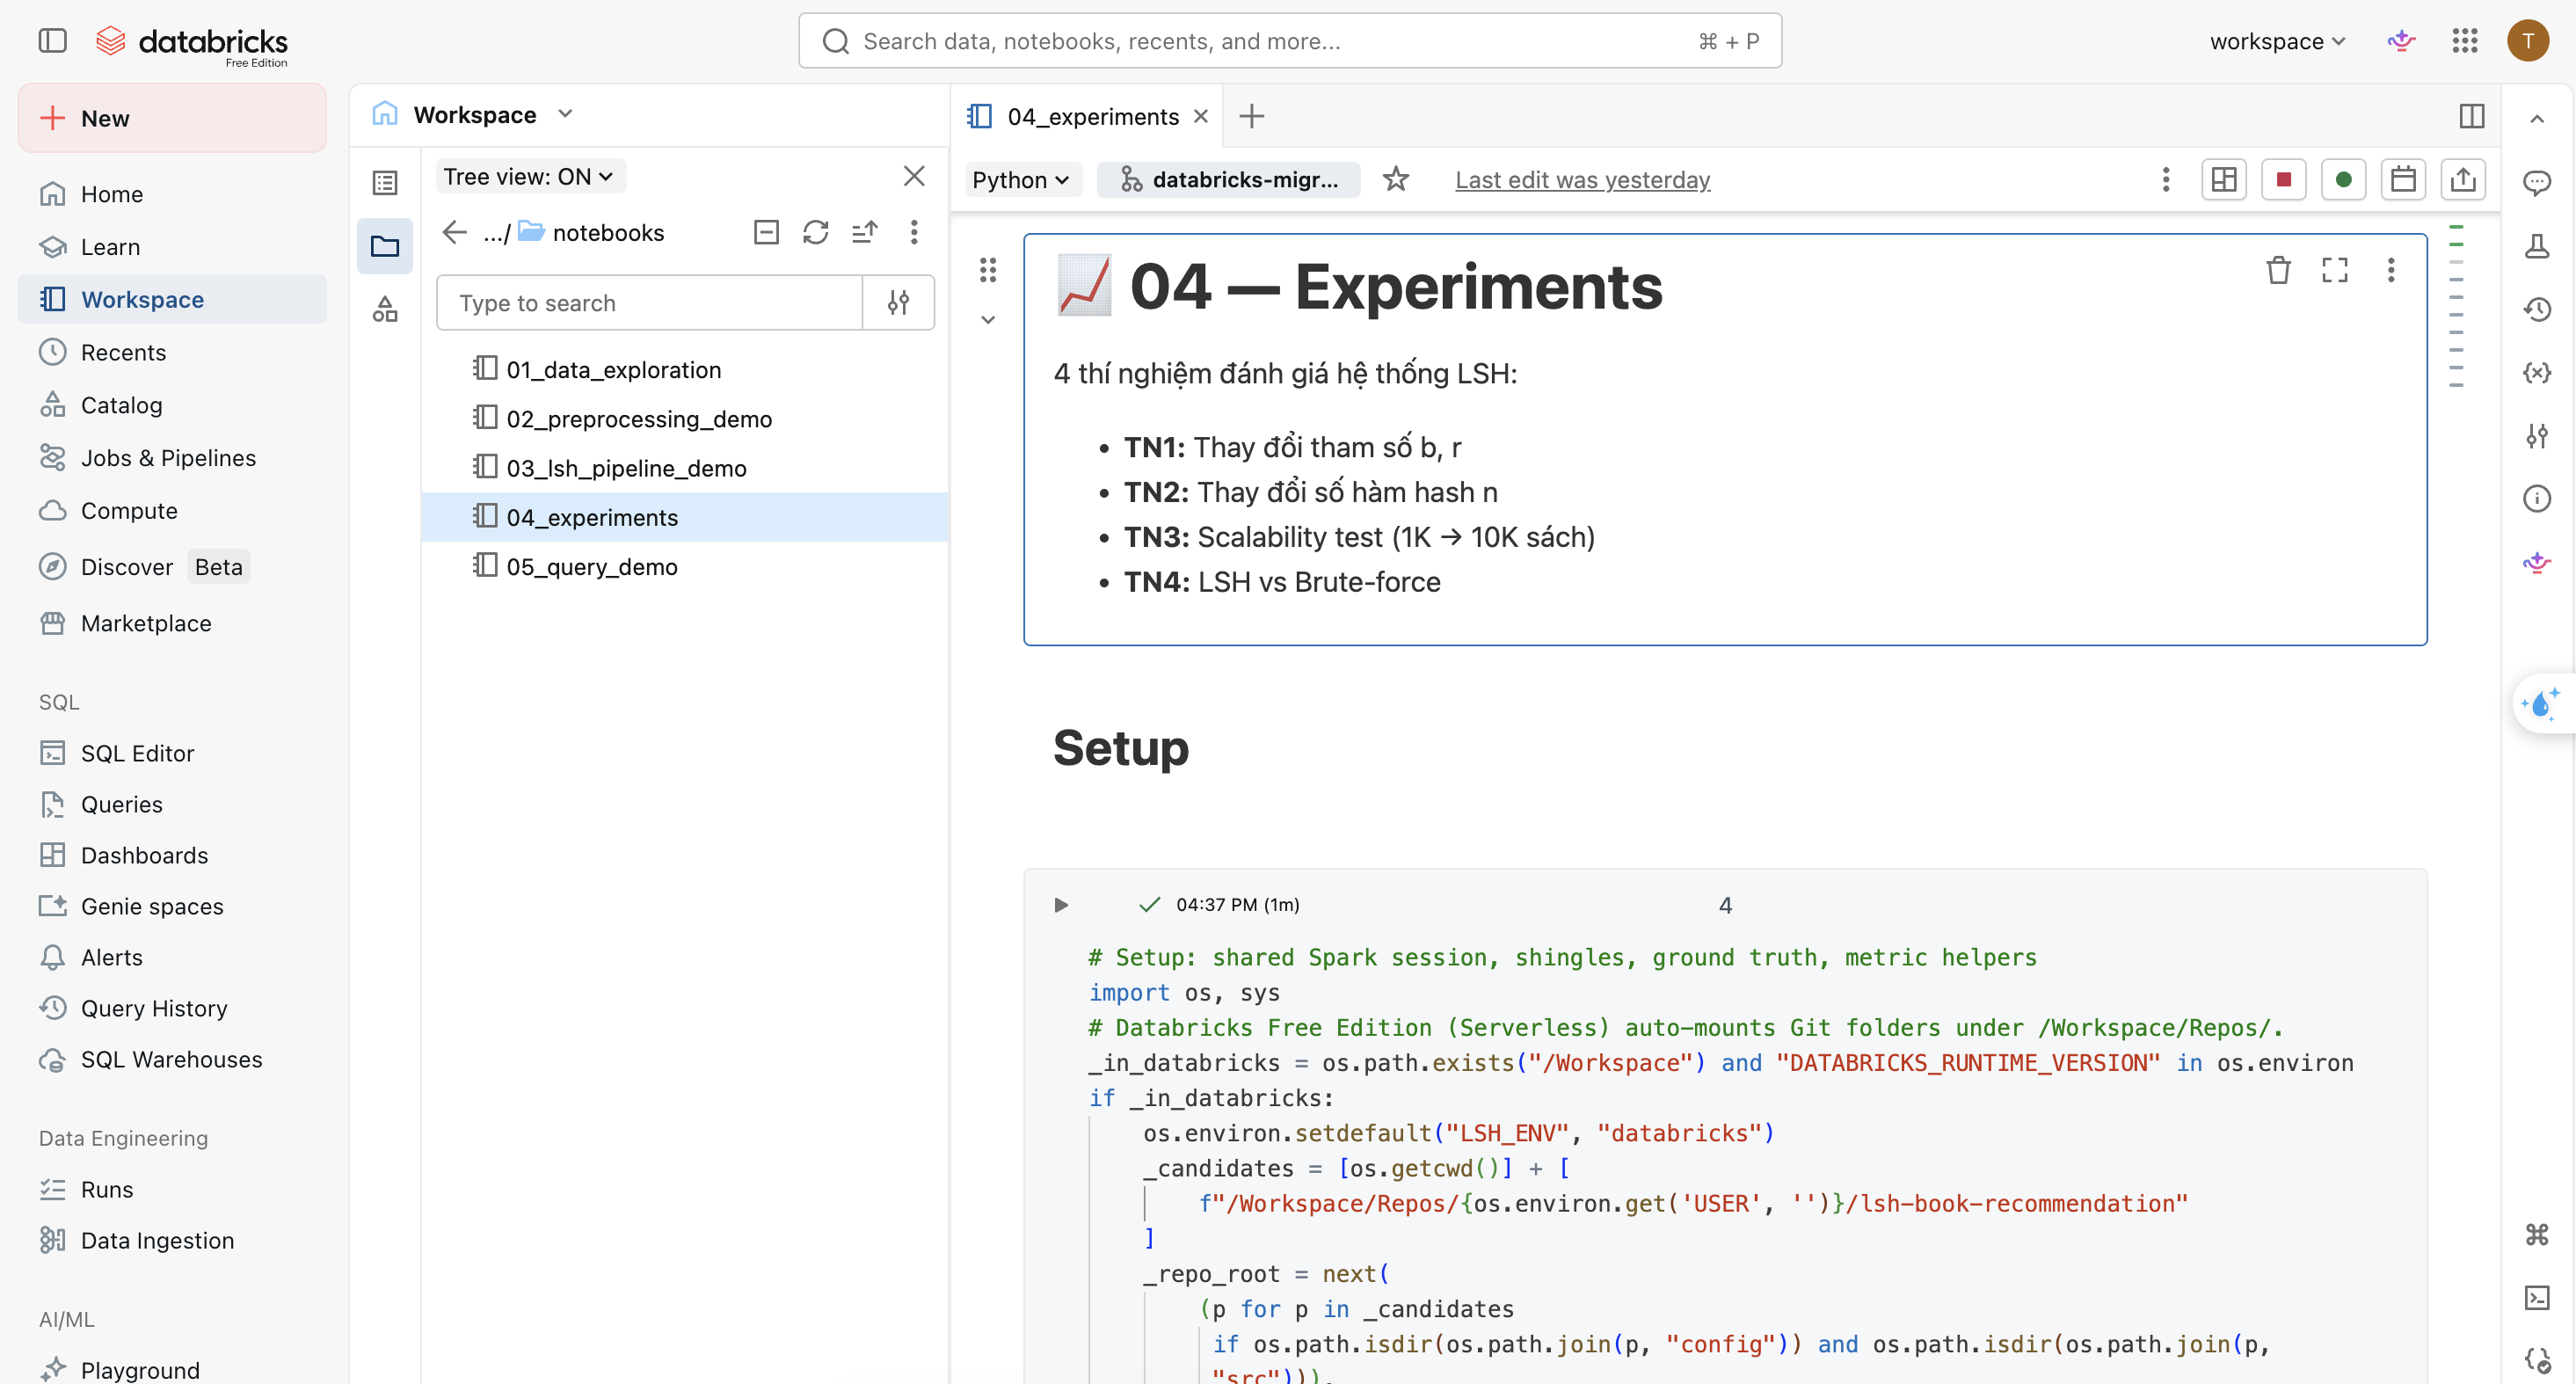
\includegraphics[height=1.1cm]{databricks.png}\hspace{0.6cm}
    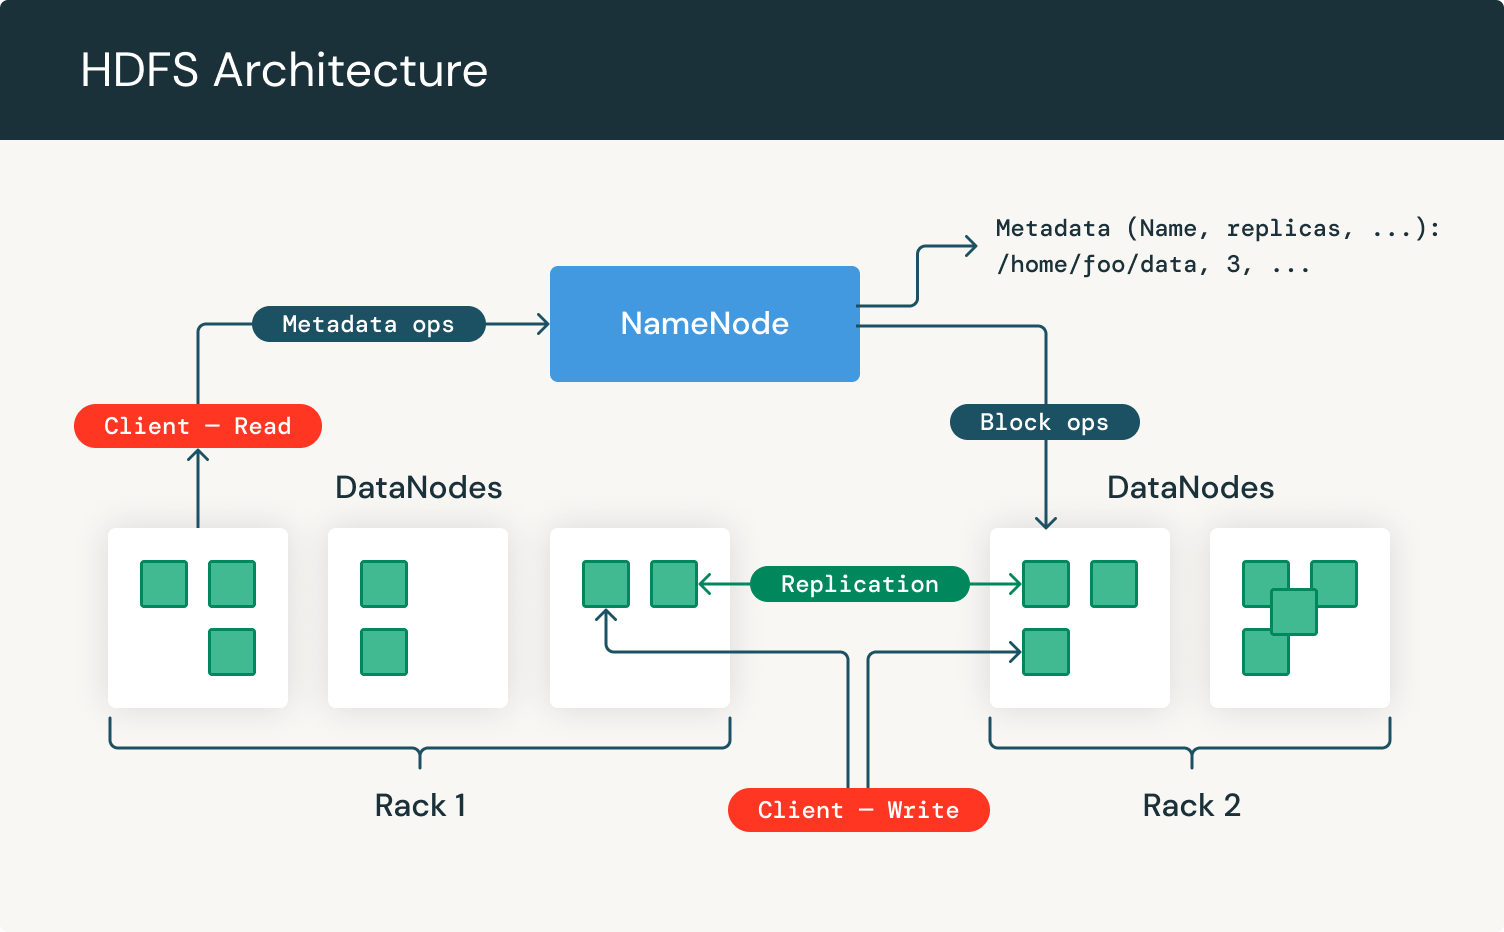
\includegraphics[height=1.1cm]{hadoop_hdfs.png}\hspace{0.6cm}
    
\includegraphics[height=1.1cm]{parquet.png}\hspace{0.6cm}
    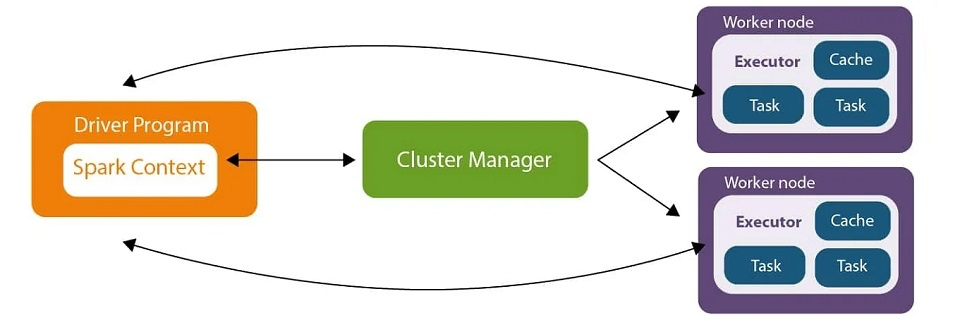
\includegraphics[height=1.1cm]{spark.png}
  \end{center}
\end{frame}

% ============================================================
% PART 2 --- [Thành viên 2]: Thuật toán & Metric Framework
% ============================================================
\begin{frame}[plain]
  \vfill
  \centering
  {\Huge\color{hcmutblue}\textbf{Phần 2}}\par
  \vspace{0.5em}
  {\Large Thuật toán LSH \& Metric Framework}\par
  \vspace{1em}
  {\large Trình bày: \textbf{[Tên thành viên 2]}}\par
  \vfill
\end{frame}

\section{Shingling}

\begin{frame}{Bước 1 --- Shingling (k-gram)}
  Mỗi tài liệu $\rightarrow$ \textbf{tập hợp k-shingle} (chuỗi $k$ từ liên tiếp).

  Project chọn \textbf{word-level trigram} ($k=3$) --- cân bằng giữa granularity và hiệu quả.

  \vfill
  \textbf{Ví dụ:} ``the quick brown fox jumps'' $\rightarrow$
  \begin{itemize}
    \item \texttt{(the, quick, brown)}
    \item \texttt{(quick, brown, fox)}
    \item \texttt{(brown, fox, jumps)}
  \end{itemize}

  \vfill
  \textbf{Output:} Parquet với schema \texttt{[book\_id, shingles: array<string>]}.
\end{frame}

\section{MinHash}

\begin{frame}{Bước 2 --- MinHash Signatures}
  Ước lượng Jaccard similarity \emph{không cần} so sánh trực tiếp các tập shingle.

  \textbf{Ý tưởng:} dùng $n$ hàm hash $h_i(x) = (a_i \cdot x + b_i) \bmod p$, lấy
  $$\mathrm{sig}_i(A) = \min_{x \in A} h_i(x).$$

  \textbf{Tính chất quan trọng:}
  $$P\bigl(\mathrm{sig}_i(A) = \mathrm{sig}_i(B)\bigr) = J(A, B) = \frac{|A \cap B|}{|A \cup B|}.$$

  \vfill
  \begin{itemize}
    \item Chiều dài signature: $n$ giá trị nguyên (project dùng $n = 100$).
    \item Output: Parquet \texttt{[book\_id, signature: array<int>]}.
  \end{itemize}
\end{frame}

\section{LSH Banding}

\begin{frame}{Bước 3 --- LSH Banding}
  Chia signature ($n$ giá trị) thành $b$ band $\times$ $r$ row, với $n = b \cdot r$.

  \textbf{Quy tắc candidate:} hai tài liệu trở thành candidate pair nếu \textbf{trùng band ở $\geq 1$ vị trí}.

  \textbf{Ngưỡng S-curve:}
  $$t \approx \left(\frac{1}{b}\right)^{1/r}.$$

  \textbf{Ví dụ:} $n=100$, $b=20$, $r=5 \;\Rightarrow\; t \approx 0.55$.

  \vfill
  \begin{center}
  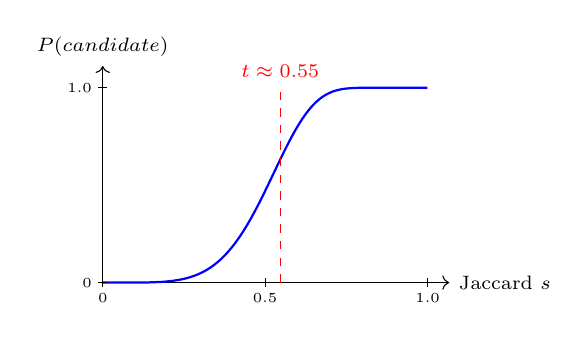
\begin{tikzpicture}[scale=0.55]
    \draw[->] (0,0) -- (8,0) node[right, font=\scriptsize] {Jaccard $s$};
    \draw[->] (0,0) -- (0,5) node[above, font=\scriptsize] {$P(\text{candidate})$};
    \draw[blue, thick, domain=0:7.5, samples=100] plot (\x, {4.5*(1-(1-(\x/7.5)^5)^20)});
    \draw[red, dashed] (4.1,0) -- (4.1,4.5) node[above, font=\scriptsize] {$t \approx 0.55$};
    \foreach \x/\l in {0/0, 3.75/0.5, 7.5/1.0}
      \draw (\x,-0.1) -- (\x,0.1) node[below=2pt, font=\tiny] {\l};
    \foreach \y/\l in {0/0, 4.5/1.0}
      \draw (-0.1,\y) -- (0.1,\y) node[left=2pt, font=\tiny] {\l};
  \end{tikzpicture}
  \end{center}
\end{frame}

\section{Query Top-K}

\begin{frame}{Bước 4 --- Query Top-K}
  \begin{center}
  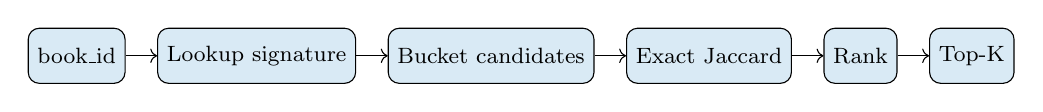
\begin{tikzpicture}[node distance=0.4cm, every node/.style={font=\footnotesize, rounded corners, fill=hcmutblue!15, draw, minimum height=0.7cm}]
    \node (a) {book\_id};
    \node[right=of a] (b) {Lookup signature};
    \node[right=of b] (c) {Bucket candidates};
    \node[right=of c] (d) {Exact Jaccard};
    \node[right=of d] (e) {Rank};
    \node[right=of e] (f) {Top-K};
    \draw[->] (a) -- (b);
    \draw[->] (b) -- (c);
    \draw[->] (c) -- (d);
    \draw[->] (d) -- (e);
    \draw[->] (e) -- (f);
  \end{tikzpicture}
  \end{center}

  \vfill
  \textbf{Tính chất:}
  \begin{itemize}
    \item Bucket lookup: $O(b)$ thay cho $O(N)$ của brute-force.
    \item Exact Jaccard chỉ tính trên candidate (selectivity $\ll 1$).
    \item LSH \emph{xấp xỉ} $\rightarrow$ False Negative (cặp similar bị bỏ sót), False Positive (cặp không similar nhưng vào candidate).
  \end{itemize}
\end{frame}

\section{Metric Framework}

\begin{frame}{4 nhóm metric đánh giá}
  \footnotesize
  \begin{tabular}{@{}lp{8cm}@{}}
    \toprule
    \textbf{Nhóm} & \textbf{Metric tiêu biểu} \\
    \midrule
    Chất lượng     & Recall, Precision, F1 (so với GT brute-force) \\
    Hiệu năng      & Execution Time, Speedup Ratio, Scalability \\
    LSH-specific   & False Positive Rate, \textbf{Selectivity}, Bucket Imbalance \\
    Dataset rep.   & GT Positive Density, Similarity Distribution, Threshold Sensitivity \\
    \bottomrule
  \end{tabular}

  \vfill
  \textbf{Ground truth:} brute-force pairwise Jaccard ở threshold $t = 0.5$.
\end{frame}

\section{Setup thí nghiệm}

\begin{frame}{Setup TN1--TN4}
  \begin{itemize}
    \item \textbf{Dataset:} 90 sách Project Gutenberg (English plain text).
    \item \textbf{Tổng cặp khả dĩ:} $\binom{90}{2} = 4{,}005$.
    \item \textbf{Ground-truth pairs ($J \geq 0.5$):} \textbf{4 cặp}.
    \item \textbf{Brute-force GT compute:} 15.73s.
    \item \textbf{Runtime:} Databricks Free Edition Serverless.
    \item \textbf{Code reuse:} \texttt{src/shingling.py}, \texttt{src/minhash.py}, \texttt{src/lsh.py}.
  \end{itemize}

  \vfill
  \textbf{4 thí nghiệm:}
  \begin{enumerate}
    \item TN1 --- Sweep tham số $(b, r)$, cố định $n = 100$.
    \item TN2 --- Sweep số hàm hash $n$, cố định $r = 5$.
    \item TN3 --- Scalability với synthetic duplication ($N \in \{200, 500, 1000\}$).
    \item TN4 --- LSH vs Brute-force toàn diện trên 90 sách.
  \end{enumerate}
\end{frame}

\section{Bảng tổng hợp 4 thí nghiệm}

\begin{frame}{Bảng tổng hợp 4 thí nghiệm}
  \scriptsize
  \begin{tabular}{@{}p{1.4cm}p{4.5cm}p{6cm}@{}}
    \toprule
    \textbf{TN} & \textbf{Biến / Setup} & \textbf{Kết quả tóm tắt} \\
    \midrule
    TN1 & $(b,r) \in \{(10,10),(20,5),(25,4),(50,2)\}$ & F1 $= 1.0$ mọi cấu hình; thời gian $\sim 1{,}260$s \\
    \midrule
    TN2 & $n \in \{50,100,150,200\}$, $r{=}5$ & F1 $= 1.0$; thời gian $\propto n$ ($\approx 12.3$s/unit) \\
    \midrule
    TN3 & Synthetic $N \in \{200,500,1000\}$ & Speedup vs BF: $0.006 \rightarrow 0.018$ \\
    \midrule
    TN4 & 90 sách, $n{=}100$, $b{=}20$, $r{=}5$ & LSH $1257.7$s vs BF $13.3$s; speedup $0.011\times$ \\
    \bottomrule
  \end{tabular}

  \vfill
  \footnotesize
  \textbf{Quan sát chính:}
  \begin{itemize}
    \item Quality metrics \emph{bão hòa} ở $1.0$ (do GT chỉ có 4 cặp / 4005).
    \item Speedup $< 1$ $\rightarrow$ \textbf{vùng overhead-dominated} của LSH ở scale này.
    \item Đường cong TN3 \emph{dốc lên} $\rightarrow$ điểm hòa vốn nằm ngoài quy mô đo được.
  \end{itemize}
\end{frame}

% ============================================================
% PART 3 --- [Thành viên 3]: Kết quả & Bài học
% ============================================================
\begin{frame}[plain]
  \vfill
  \centering
  {\Huge\color{hcmutblue}\textbf{Phần 3}}\par
  \vspace{0.5em}
  {\Large Kết quả thí nghiệm \& Bài học}\par
  \vspace{1em}
  {\large Trình bày: \textbf{[Tên thành viên 3]}}\par
  \vfill
\end{frame}

\section{TN1 --- Sweep $(b, r)$}

\begin{frame}{TN1 --- Sweep tham số $(b, r)$, $n = 100$}
  \scriptsize
  \begin{tabular}{@{}lcccccc@{}}
    \toprule
    Config & $b$ & $r$ & $t^{*}$ & $|$cand$|$ & F1 & Time (s) \\
    \midrule
    $b{=}10, r{=}10$ & 10 & 10 & 0.7943 & 4 & 1.0 & 1258.504 \\
    $b{=}20, r{=}5$  & 20 & 5  & 0.5493 & 4 & 1.0 & 1260.754 \\
    $b{=}25, r{=}4$  & 25 & 4  & 0.4472 & 4 & 1.0 & 1263.613 \\
    $b{=}50, r{=}2$  & 50 & 2  & 0.1414 & 4 & 1.0 & 1259.748 \\
    \bottomrule
  \end{tabular}

  \begin{center}
    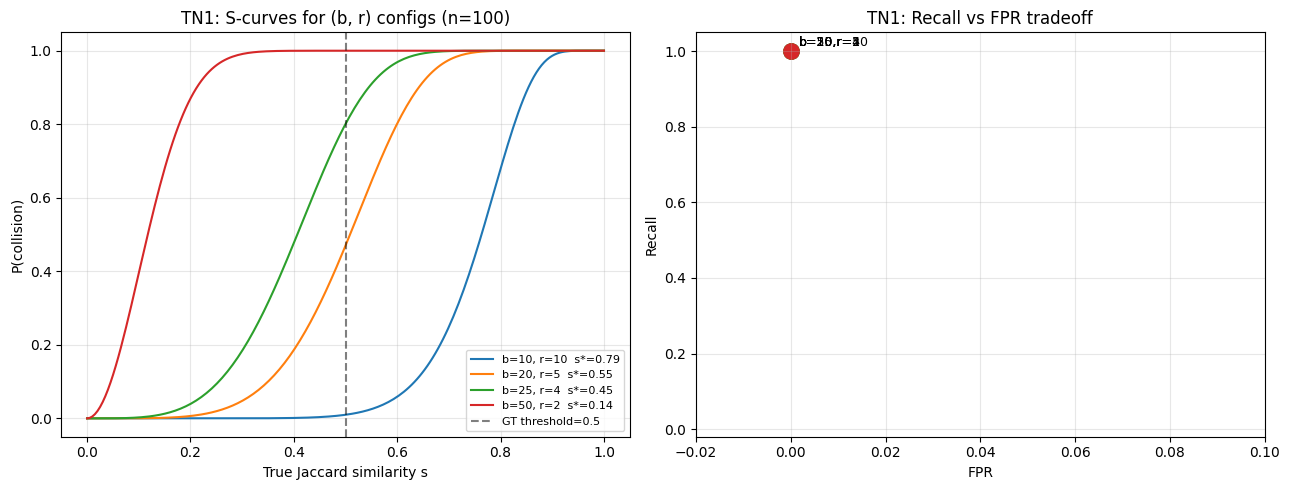
\includegraphics[height=4cm]{tn1_scurve_recallfpr.png}
  \end{center}

  \tiny\textbf{Diễn giải:} Cấu hình $b{=}20, r{=}5$ ($t^{*} \approx 0.55$) gần GT ($0.5$) nhất; mọi cấu hình đều F1 $= 1.0$ trên dataset 90 sách (metric bão hòa).
\end{frame}

\section{TN2 --- Sweep $n$}

\begin{frame}{TN2 --- Sweep số hàm hash $n$, $r = 5$ cố định}
  \scriptsize
  \begin{tabular}{@{}cccccc@{}}
    \toprule
    $n$ & $b$ & $r$ & $|$cand$|$ & F1 & Time (s) \\
    \midrule
    50  & 10 & 5 & 4 & 1.0 & 641.383  \\
    100 & 20 & 5 & 4 & 1.0 & 1254.736 \\
    150 & 30 & 5 & 4 & 1.0 & 1870.203 \\
    200 & 40 & 5 & 4 & 1.0 & 2491.090 \\
    \bottomrule
  \end{tabular}

  \begin{center}
    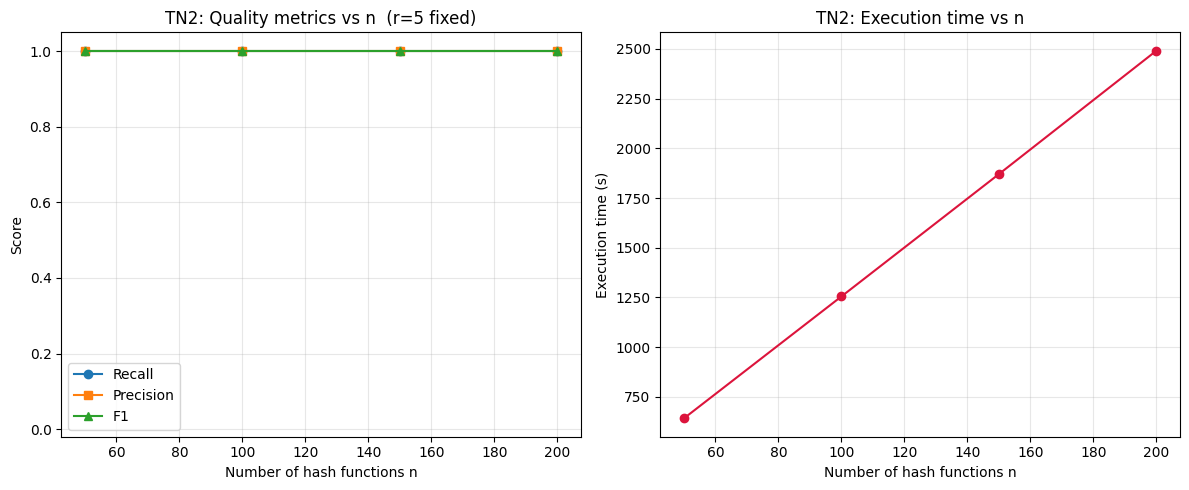
\includegraphics[height=4cm]{tn2_quality_time_vs_n.png}
  \end{center}

  \tiny\textbf{Diễn giải:} Thời gian tăng tuyến tính với hệ số $\approx \mathbf{12.3}$\textbf{s/hash unit}; F1 đã bão hòa từ $n = 50$ $\rightarrow$ không có lý do thực nghiệm chọn $n > 100$.
\end{frame}

\section{TN3 --- Scalability}

\begin{frame}{TN3 --- Scalability test}
  \scriptsize
  \begin{tabular}{@{}rrrrrr@{}}
    \toprule
    Size & $T_{\text{sig}}$ & $T_{\text{LSH}}$ & $T_{\text{BF}}^{(5\,\text{queries})}$ & $|$cand$|$ & Speedup \\
    \midrule
    200  & 7.572 & 663.589  & 4.179  & 217  & 0.006 \\
    500  & 8.172 & 1622.356 & 9.424  & 1354 & 0.006 \\
    1000 & 7.622 & 3224.083 & 59.019 & 5916 & 0.018 \\
    \bottomrule
  \end{tabular}

  \begin{center}
    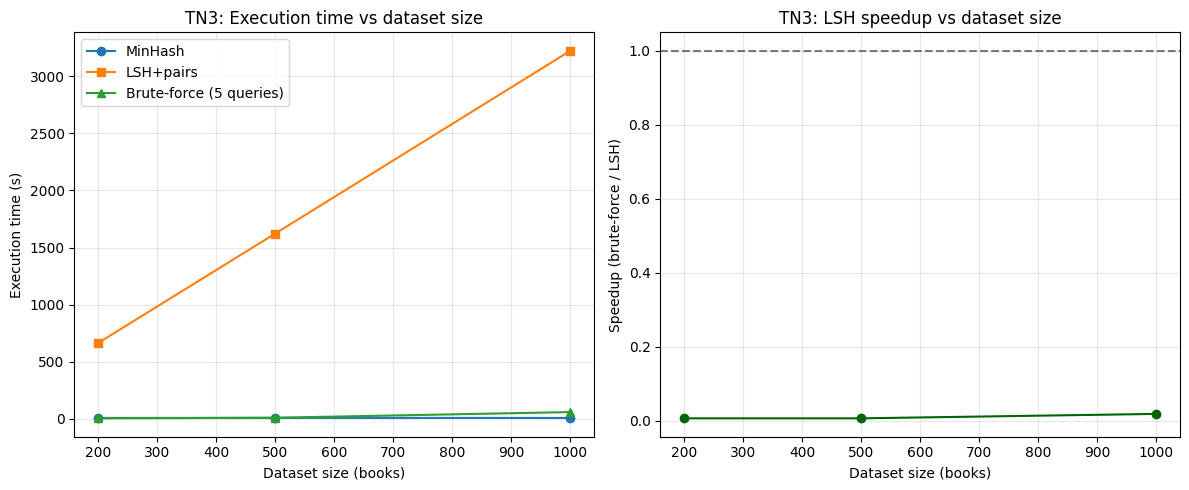
\includegraphics[height=3.7cm]{tn3_time_speedup_vs_size.png}
  \end{center}

  \tiny\textbf{Diễn giải:} Speedup tăng $0.006 \rightarrow 0.018$ ($3\times$) khi $N$ tăng $5\times$ $\rightarrow$ điểm hòa vốn nằm ở $N \gg 1{,}000$ (Free Edition driver memory không cho test cao hơn).
\end{frame}

\section{TN4 --- LSH vs Brute-force}

\begin{frame}{TN4 --- LSH vs Brute-force toàn diện}
  90 sách, $n = 100$, $b = 20$, $r = 5$, $t = 0.5$:

  \scriptsize
  \begin{tabular}{@{}lcccccrr@{}}
    \toprule
    Method & Recall & Prec & F1 & FPR & \textbf{Selectivity} & $|$cand$|$ & Time (s) \\
    \midrule
    LSH        & 1.0 & 1.0 & 1.0 & 0.0 & \textbf{0.001} & 4    & 1257.727 \\
    BruteForce & 1.0 & 1.0 & 1.0 & 0.0 & 1.000          & 4005 & 13.306   \\
    \bottomrule
  \end{tabular}

  \vfill
  \normalsize\textbf{Speedup (BF / LSH) $= 0.011\times$.}

  \vfill
  \textbf{Hai cách đọc kết quả:}
  \begin{itemize}
    \item \emph{Selectivity:} LSH lọc $4{,}005 \rightarrow 4$ candidate ($1000\times$ giảm) --- \textbf{LSH thắng tuyệt đối}.
    \item \emph{Wall time:} LSH chậm hơn $\sim 95\times$ --- \textbf{overhead Spark/JVM chi phối ở $N = 90$}.
  \end{itemize}

  \footnotesize Theo TN3, điểm hòa vốn về wall time nằm ở $N \gg 1000$.
\end{frame}

\section{Hạn chế}

\begin{frame}{Hạn chế của thí nghiệm}
  \textbf{Dataset:}
  \begin{itemize}
    \item \textbf{(H1)} Chỉ \textbf{4 cặp GT} ($J \geq 0.5$) trong 4005 cặp $\rightarrow$ quality metrics bão hòa, không phân biệt được giữa cấu hình.
    \item \textbf{(H2)} Spark/JVM overhead chi phối ở scale nhỏ (TN1 thời gian gần như không đổi $1258 \pm 3$s).
    \item \textbf{(H3)} Threshold $J \geq 0.5$ quá khắc nghiệt --- corpus đa thể loại Gutenberg trung bình $J < 0.1$.
  \end{itemize}

  \vfill
  \textbf{Hạ tầng (pivot Databricks Free Edition):}
  \begin{itemize}
    \item Driver memory hẹp $\rightarrow$ TN3 cắt từ $\{1\text{K},3\text{K},5\text{K},10\text{K}\}$ xuống $\{200, 500, 1000\}$.
    \item Không truy cập \texttt{spark.sparkContext}; \texttt{PERSIST TABLE} bị từ chối.
    \item Compute dùng chung $\rightarrow$ Spark warm-up + shuffle dominate timing.
  \end{itemize}
\end{frame}

\section{Hướng phát triển}

\begin{frame}{Hướng phát triển}
  \textbf{Hạ tầng:}
  \begin{itemize}
    \item Khi xin được credits: cluster $\geq 3$ worker, $\geq 16$GB driver $\rightarrow$ chạy lại TN3 ở $5{,}000$--$10{,}000$ sách để cắt qua điểm hòa vốn.
    \item Migrate sang HDFS thật (đường dẫn đã thiết kế --- Section 4 Listing).
  \end{itemize}

  \vfill
  \textbf{Phương pháp đánh giá:}
  \begin{itemize}
    \item Mở rộng dataset thật $\geq 2{,}000$ sách Gutenberg.
    \item Tạo positives nhân tạo có gradient $J \in \{0.3, 0.5, 0.7, 0.9\}$.
    \item Tách $T_{\text{setup}}$ vs $T_{\text{algo}}$ trong code đo $\rightarrow$ speedup công bằng.
  \end{itemize}

  \vfill
  \textbf{Triển khai sản phẩm:}
  \begin{itemize}
    \item Tầng query real-time (LSH index in-memory, $O(b)$ bucket lookup).
    \item Hoàn thiện FastAPI + Streamlit (đã thiết kế, chưa implement).
  \end{itemize}
\end{frame}

\section{Kết luận}

\begin{frame}{Kết luận}
  \begin{itemize}
    \item Triển khai pipeline LSH end-to-end: Shingling $\rightarrow$ MinHash $\rightarrow$ Banding $\rightarrow$ Query Top-K.
    \item Pivot \textbf{HDFS+Spark $\rightarrow$ Databricks Free Edition Serverless} --- giải pháp pragmatic khi không có cloud credits.
    \item TN1, TN2 cho thấy hệ thống \emph{đúng chức năng} (F1 $= 1.0$); TN3, TN4 cho thấy hệ thống đang ở \textbf{vùng overhead-dominated} của LSH.
    \item Đường cong scalability TN3 dốc lên $\rightarrow$ tại $N \gg 1{,}000$, LSH sẽ thắng brute-force về wall time, không chỉ selectivity.
  \end{itemize}

  \vfill
  \begin{center}
  {\Large\textbf{Cảm ơn quý thầy cô và các bạn!}}\\[0.6em]
  {\large Q\&A}
  \end{center}
\end{frame}

\end{document}
